%%%%%%%%%%%%%%%%%%%%%%%%%%%%%%%%%%%%%%%%%
% Lachaise Assignment
% LaTeX Template
% Version 1.0 (26/6/2018)
%
% This template originates from:
% http://www.LaTeXTemplates.com
%
% Authors:
% Marion Lachaise & François Févotte
% Vel (vel@LaTeXTemplates.com)
%
% License:
% CC BY-NC-SA 3.0 (http://creativecommons.org/licenses/by-nc-sa/3.0/)
% 
%%%%%%%%%%%%%%%%%%%%%%%%%%%%%%%%%%%%%%%%%

%----------------------------------------------------------------------------------------
%	PACKAGES AND OTHER DOCUMENT CONFIGURATIONS
%----------------------------------------------------------------------------------------

\documentclass{article}
\usepackage{amsthm}
\usepackage{listings}
\usepackage{xcolor}
\usepackage{graphicx}


\lstset{
	language=Python,
	basicstyle=\ttfamily\small,
	keywordstyle=\color{blue},
	stringstyle=\color{red},
	commentstyle=\color{purple},
	showstringspaces=false,
	numbers=left,
	numberstyle=\tiny\color{gray},
	breaklines=true,
	frame=single,
	captionpos=b
}
\newtheorem{definition}{Definition}[section]

\input{structure.tex} % Include the file specifying the document structure and custom commands

%----------------------------------------------------------------------------------------
%	ASSIGNMENT INFORMATION
%----------------------------------------------------------------------------------------

\title{Transformers Breakdown: Sinusoidal Embeddings} % Title of the assignment

\author{Giovani Tavares\\ \texttt{giovanitavares@outlook.com}} % Author name and email address

\date{University of Sao Paulo --- \today} % University, school and/or department name(s) and a date

%----------------------------------------------------------------------------------------

\begin{document}

\maketitle % Print the title

%----------------------------------------------------------------------------------------
%	INTRODUCTION
%----------------------------------------------------------------------------------------

\section*{Motivation} % Unnumbered section

I've been studying and using Transformer models for a while now. While I have a good understanding of their components, the mathematical intricacies of some remain unclear. Therefore, I decided to write a series of Medium posts to help you grasp some important concepts visually. The first of such concept is Sinusoidal Embeddings.


%----------------------------------------------------------------------------------------
%	PROBLEM 1
%----------------------------------------------------------------------------------------

\section{Sinusoidal Embeddings - An Overview}
\subsection{What are Sinusoidal Embeddings for?} % Numbered section

As we know, embeddings are vectors that represent an input sentence for a transformer model. Embeddings are vectors that represent an input sentence for a transformer model. Beyond capturing and learning a sentence's intrinsic semantics, it is crucial for the language model to be able to learn the relationship between a token's position within a larger sentence and its semantics. To understand why, consider the example below:

\begin{itemize}
	\item \textbf{Sentence I:} The chef, \textit{who had prepared the meal with great care}, served the dish to the guests.
	\item \textbf{Sentence II:} The chef served the dish to the guests, \textit{who had prepared the meal with great care}.
	
\end{itemize}

Notice how the meaning of the clause \textit{"who had prepared the meal with great care"} changes between the sentences. In \textbf{Sentence I}, it refers to the chef, while in \textbf{Sentence II}, it refers to the guests.

This significant difference in meaning is entirely dependent on the clause's position within the sentences. The semantics of a clause within a sentence is heavily influenced its position within the sentence. Therefore, it is essential for transformer models to encode positional information in their input representations. This is one of the key roles of the Sinusoidal Embedding function, which takes as input a sequence of tokens and outputs the position-informed embedding for such sequence.

%------------------------------------------------


\subsection{What Properties Should Sinusoidal Embeddings (SE) Should Apply?}

\begin{enumerate}
	\item \textbf{Periodicity:} the model trained with sinusoidal embeddings should be able to capture the relative positions of tokens effectively, which means that the distances between the embeddings of a pair of clauses should not depend on their absolute position within the longer sentence. This is achieved by making the sinusoidal embeddings functions periodic, which was to be expected from the name of the function. 
	\item \textbf{Unique Representation (Injective Function):} this one is straight forward from the fact that  sinusoidal embeddings must represent the positions of tokens within a sentence. This means that sets of tokens in different positions should not be mapped to the same output, otherwise different positions would have the same representation.
	\item \textbf{Scale Invariance:} sinusoidal embeddings should represent tokens positions consistently regardless of the sequence length. This property is crucial for handling sequences of varying lengths in a transformer model including those that are longer than the ones the model were trained on. Essentialy, the scale invariance property says that the distance of two inputs $x_t$ and $x_{t - k}$ should be similar among different values of $t$. In other words, $x_t - x_{t - k}$ should not depend on $t$.
	\item \textbf{Linearity:} this property is somewhat related to the scale invariance property. For the Sinusoidal Embedding function to be linear is good, because functions having such property are more easily learned by neural networks. Moreover, if the Sinusoidal Embedding Function is linear we also achieve the scale invariance property. This is true, because if such Sinusoidal Embedding function ($SE$) is linear, for any pair of sets of tokens separated by a distance of $k$, say $X_t, X_{t+k}$, there is a linear transformation $M$ such that $M \times SE(X_t) = SE(X_{t+k})$. Hence, in order to represent $X_{t+k}$,  the model must only learn the linear transformation $M$ regardless of the value of $k$. 
\end{enumerate}


\subsection{How are Sinusoidal Embeddings Defined?}

The author's of the \textit{Attention is All You Need} paper define the Sinusoidal Embeddings Function ($SE$) like the following.

\begin{definition}[Sinusoidal Embeddings]
	\label{def:sin_embedding}
	
	For a position \( pos \) in the sequence and a dimension \( i \) (where \( i \) ranges from 0 to \( \frac{d}{2}-1 \)), the sinusoidal embedding ($SE$) function is given by:
	
	\begin{align}
		SE_{(pos, 2i)} &= \sin\left(\frac{pos}{10000^{\frac{2i}{d}}}\right) \\
		SE_{(pos, 2i+1)} &= \cos\left(\frac{pos}{10000^{\frac{2i}{d}}}\right) \\
	\end{align}
	
	This function can be vectorially expressed as the following: 
	\begin{align}
		\mathbf{SE}(pos) &= \left[ \sin\left(pos \cdot e^{- \frac{2i \ln(10000)}{d}}\right), \cos\left(pos \cdot e^{- \frac{2i \ln(10000)}{d}}\right) \right]_{i=0}^{\frac{d}{2}-1}
	\end{align}
	

\end{definition}

where:

\begin{itemize}
	\item \( pos \) is the position in the sequence.
	\item  \( i \) is the dimension index.
	\item  \( d \) is the dimensionality of the embeddings.
\end{itemize}


Notice that $SE$ is essentialy a function that outputs $sin$ values to the even dimensions of an input $x_t$ and $cos$ for the odd ones with exponentially decreasing frequencies.


In the next section we will use the definition of  $SE$ function to verify the validity of the previous $4$ properties it should have. Some verification will be done analitically and others will be done using $Python$.

\section{Properties Verification}

In this section, we will be checking each of the $4$ presented properties of the oidal Embeddings using analytical techniques.


\subsection{Peridiocity}

This peridiocity of the $SE$ function is straight-forward. Different dimensions $i$ and $i+k$ of an input  $x_t \in \mathbb{R}^{d}$ with position $pos$ will have the same values output by the $sin$ and $cos$ because such functions are periodic. 

\begin{info} % Information block
	One question that a reader might have is whether the peridiocity property does not contradict the injectivity one. The answer for that is no. The peridiocity property is observed at a single dimension level, which means $SE_{(pos, 2i)}$ that outputs a single value, is be periodic. The injectivity, on the other hand, is observed at the entire embedding level, which means $SE_{(pos)}$, that outputs a vector (embedding) of dimension $d$ is injective.
\end{info}


\subsection{Unique Representation (Injective Function)}

We are gonna prove that two sequences from different positions are \textbf{not} mapped to the same vector/output, using a \textit{proof by contradiction}. 
Let's assume that two sequences $x_{t_1}$ and $x_{t_2}$, with different positions $t_1$ and $t_2$, respectivelly, are mapped to the same output using the previously  $SE$ function. This assumption implies the following \textbf{for any dimension i}

\begin{align}
	SE(x_{t_1}) = SE(x_{t_2}) & \implies SE(t_1, 2i) = SE(t_2, 2i) \text{   and   }SE(t_1, 2i+1) = SE(t_2, 2i+1) \\
	 \implies \sin\left(\frac{t_1}{10000^{\frac{2i}{d}}}\right) &= \sin\left(\frac{t_2}{10000^{\frac{2i}{d}}}\right) \text{   and   }\cos\left(\frac{t_1}{10000^{\frac{2i}{d}}}\right) = \cos\left(\frac{t_2}{10000^{\frac{2i}{d}}}\right) 
\end{align}


For the last implication to be true, either the arguments of the $sin$ and $cos$ functions are the exact same or they are separated by $2\pi k$. We know they are not the same, because $t_1 \neq t_2$. Therefore, we're left with the condition:


\begin{align}
	| \frac{t_1}{10000^{\frac{2i}{d}}} - \frac{t_2}{10000^{\frac{2i}{d}}} | &=  2\pi k \\
	\implies 	| \frac{t_1 - t_2}{10000^{\frac{2i}{d}}} | &=  2\pi k \\
	\implies 	| t_1 - t_2 | &=  2\pi k 10000^{\frac{2i}{d}}  \text{       [contradiction]} \\ 
\end{align}


Since \( t_1 \) and \( t_2 \) are integers that represent the sequences positions, and \( 10000^{\frac{2i}{d}} \) is a positive real number, the right side of the equation \( \left| t_1 - t_2 \right| = 2\pi k \cdot 10000^{\frac{2i}{d}} \) must also be an integer. However, \( 2\pi k \cdot 10000^{\frac{2i}{d}} \) is generally not an integer because \( 2\pi \) is an irrational number, which leads us to a contradiction.

Hence, the initial assumption $SE(x_{t_1}) = SE(x_{t_2})$ must be false, which let's us say that \textbf{ two sequences $x_{t_1}$ and $x_{t_2}$, with different positions $t_1$ and $t_2$, respectivelly, are not mapped to the same output using the previously  $SE$ function}.


\subsection{Linearity \& Scale Invariance}

As previously mentioned, the scale invariance property is a consequence of $SE(pos)$'s linearity. Hence, by proving that $SE(pos)$ is linear we also prove that such function is scale invariant. 

We need to find $M \in \mathbb{R}^{d \times d}$ such that $M \times  SE(x_{t}) = SE(x_{t + k}) $. We have the following system of equations:

\begin{align}
	\begin{bmatrix}
		m_{00} & m_{01} & \cdots & m_{0(d-1)} \\
		m_{10} & m_{11} & \cdots & m_{1(d-1)} \\
		\vdots & \vdots & \ddots & \vdots \\
		m_{(d-1) 0} & m_{(d-1)1} & \cdots & m_{(d-1)(d-1)}
	\end{bmatrix}
	\begin{bmatrix}
		sin(\omega_0 t) \\
		cos(\omega_0 t) \\
		\vdots \\
		sin(\omega_{(d-2)/2} t) \\
		cos(\omega_{(d-2)/2} t) 
	\end{bmatrix}
	&=\begin{bmatrix}
		sin(\omega_0 (t+k)) \\
		cos(\omega_0 (t+k)) \\
		\vdots \\
		sin(\omega_{(d-2)/2}  (t+k)) \\
		cos(\omega_{(d-2)/2} (t+k)) 
	\end{bmatrix}
\end{align}

\begin{align}
	m_{00}\sin(\omega_0 t) + m_{01}\cos(\omega_0 t) + \cdots + m_{0(d-1)}\cos(\omega_{d-1} t) &= \sin(\omega_0 t)\cos(\omega_0 k) + \sin(\omega_0 k)\cos(\omega_0 t) \\
	m_{10}\sin(\omega_0 t) + m_{11}\cos(\omega_0 t) + \cdots + m_{1(d-1)}\cos(\omega_{d-1} t) &= \cos(\omega_0 t)\cos(\omega_0 k) - \sin(\omega_0 k)\sin(\omega_0 t) \\
	&\vdots \nonumber \\
	m_{(d-1)0}\sin(\omega_0 t) + m_{(d-1)1}\cos(\omega_0 t) + \cdots + m_{(d-1)(d-1) }\cos(\omega_{\frac{d-2}{2}}  t) &= \cos(\omega_{\frac{d-2}{2}}  t)\cos(\omega_{\frac{d-2}{2}}  k) - \sin(\omega_{\frac{d-2}{2}}  k)\sin(\omega_{\frac{d-2}{2}}  t)
\end{align}


This system has a solution:
\begin{align}
	m_{00} &= \cos(\omega_0 k) \\
	m_{01} &= \sin(\omega_0 k) \\
	m_{02} &= m_{03} = \hdots = m_{0(d-1)} = 0 \\
	m_{10} &= -\sin(\omega_0 k) \\
	m_{11} &= \cos(\omega_0 k) \\
	m_{12} &= m_{13} = \hdots = m_{1(d-1)} = 0 \\
	m_{22} &= \cos(\omega_1 k) \\
	m_{23} &= \sin(\omega_1 k) \\
	m_{20} &= m_{21} = m_{24} = \hdots = m_{2(d-1)} = 0 \\
	m_{32} &= -\sin(\omega_1 k) \\
	m_{33} &= \cos(\omega_1 k) \\
	m_{30} &= m_{31} = m_{34} = \hdots = m_{3(d-1)} = 0 \\
	& \vdots \nonumber \\
	m_{(d-2)(d-2)} &= \cos(\omega_{(d-2)/2} k) \\
	m_{(d-2)(d-1)} &= \sin(\omega_{(d-2)/2} k) \\
	m_{(d-2)0} &= m_{(d-2)1} = m_{(d-2)2} = \hdots = m_{(d-2)(d-3)} = 0 \\
	m_{(d-1)(d-2)} &= -\sin(\omega_{(d-2)/2} k) \\
	m_{(d-1)(d-1)} &= \cos(\omega_{(d-2)/2} k) \\
	m_{(d-1)0} &= m_{(d-1)1} = m_{(d-1)2} = \hdots = m_{(d-1)(d-3)} = 0 \\
\end{align}

Which lets us define $M$ as:

\begin{align}
	M &=
	\begin{bmatrix}
		\cos(\omega_0 k) & \sin(\omega_0 k) & 0 & 0 & \cdots & 0 & 0 \\
		-\sin(\omega_0 k) & \cos(\omega_0 k) & 0 & 0 & \cdots & 0 & 0 \\
		0 & 0 & \cos(\omega_1 k) & \sin(\omega_1 k) & \cdots & 0 & 0 \\
		0 & 0 & -\sin(\omega_1 k) & \cos(\omega_1 k) & \cdots & 0 & 0 \\
		\vdots & \vdots & \vdots & \vdots & \ddots & \vdots & \vdots \\
		0 & 0 & 0 & 0 & \cdots & \cos(\omega_{(d-2)/2} k) & \sin(\omega_{(d-2)/2} k) \\
		0 & 0 & 0 & 0 & \cdots & -\sin(\omega_{(d-2)/2} k) & \cos(\omega_{(d-2)/2} k)
	\end{bmatrix}
\end{align}



We found a matrix $M \in \mathbb{R}^{d \times d}$ such that $M \times  SE(x_{t}) = SE(x_{t + k}) $. Hence, $SE$ is a linear function. Moreover, notice how \textbf{M does not depend on t}, only on $k$. This is what gives us the scale invariability property.

\section{Visualizing the Sinusoidal Embeddings Properties With \textit{Python}}

In this section, we will write some $Python$ functions and classes to visualize the $4$ cited properties of Sinusoidal Embeddings. Visualization is a great way to grasp such function's behaviour without having to necessarily prove it (even though you can always come back to this post with you're interested in the proofs).

\subsection{Sinusoidal Embedding Definition With Pytorch}

The sinusoidal embeddings module will store a multi-embedding tensor with $shape =  (max\_pos, embed\_dim)$, where $max\_pos$ represents the maximum position we are interested in representing. This way, each of such tensor's row represents a the sinusoidal embedding for a position $pos$ such that $SE(pos), 0 \leq pos <  max\_pos $. 


\begin{lstlisting}[caption={Sinusoidal Embedding Module Definition}]
	
import pytorch.nn as nn
	
class SinusoidalEmbeddings(nn.Module):

	def __init__(self, max_pos:int, embed_dim: int):
		super().__init__()
		# Returns a tensor with shape (time_steps, 1).
		positions = torch.arange(max_pos).unsqueeze(1).float()
		
		# Creates a tensor with shape (embed_dim //2,). We just need 
		# half of the dimensions of the input embeddings to compute all
		# of the sinusoidal embeddings frequencies
		dimensions = torch.arange(start = 0, end = embed_dim, step = 2).float()
		
		# Compute the frequencies vector
		frequencies = torch.exp(dimensions * -(math.log(10000.0) / embed_dim))
		
		# Initialize the embeddings tensor with shape (time_steps, embed_dim)
		embeddings = torch.zeros(time_steps, embed_dim, requires_grad=False)
		
		# Apply sin to even indices (0, 2, 4, ...) of the input embeddings
		embeddings[:, 0::2] = torch.sin(positions * frequencies)
		
		# Apply cos to odd indices (1, 3, 5, ...) of the input embeddings
		embeddings[:, 1::2] = torch.cos(positions * frequencies)
		
		self.embeddings = embeddings
	
	def forward(self, x, t):
		embeds = self.embeddings[t].to(x.device)
		return embeds[:, :, None, None]

\end{lstlisting}

\subsection{Sinusoidal Embeddings Periodicity}

As previously mentioned, the periodicity of  Sinusoidal Embeddings is observed in each of its dimensions. Hence, we need to plot its dimensions values for different positions to see their periodic behavior. 

\begin{lstlisting}[caption={Generating the plot of the embedding's dimensions for in different positions}]
	
max_pos = 100

# Our embeddings will only have 4 dimension
embed_dim = 4
sinusoidal_embeddings = SinusoidalEmbeddings(max_pos, embed_dim)

# Generate embeddings for a range of time steps
embeddings = sinusoidal_embeddings.embeddings

# Convert embeddings to numpy for plotting
embeddings_np = embeddings.numpy()

# Plot the sunosoidal embeddings for different time steps
plt.figure(figsize=(14, 8))
for i in range(embed_dim):
	plt.plot(embeddings_np[:, i], label=f"Dim {i} (i = {i//2})")
	
plt.title("SE(pos, 2i)")
plt.xlabel("pos")
plt.ylabel("Value")
plt.legend(loc="upper right", bbox_to_anchor=(1.15, 1))
\end{lstlisting}

\begin{figure}[h] 
	\centering
	\includegraphics[width=\linewidth]{images/sin_embeds_periodicity.png}
	\caption{The embedding's dimensions values for the $SE$ function }
	\label{fig:sin_embeds_periodicity}
\end{figure}

As noticed in the plot above, the value of the function $SE(pos, 2i)$ defined in \ref{def:sin_embedding} repeats itself in a frequency that is inversely proportional to $i$, which is the dimension being represented (an index in the multidimensional embedding). As a consequence, \textbf{the higher the dimension of our model's embeddings (previously called $d$ and called $embed\_dim$ in the Sinusoidal Embedding module), the less $SE$ values vary.} 

Intuitively, such consequence means that embeddings close to each other (they represent sentences in not very distant positions), will have their differences captured in lower dimensions, because their higher dimensions are likely to be very similar. The exact opposite is true for embeddings that represent sentences that are far away from each other. Let's visualize that by plotting high dimensional embeddings for different positions heatmaps.


\begin{lstlisting}[caption={Generating the plot of the sinusoidal embeddings for different positions}]
	
import torch

# We'll create embeddings with many dimensions to better see the 
# frequency decay effect
max_pos = 100
embed_dim = 128
sinusoidal_embeddings = SinusoidalEmbeddings(max_pos, embed_dim)

x = torch.zeros(embed_dim)
results = torch.zeros(max_pos, embed_dim)
for pos in range(max_pos):
results[pos] =  x + sinusoidal_embeddings.embeddings[pos]

tensor_np = results.numpy()
# Plot the heatmap using matplotlib
plt.figure(figsize=(16, 6))
plt.imshow(tensor_np, aspect='auto', cmap='RdBu')
plt.colorbar(label='')
plt.xlabel('2i')
plt.ylabel('pos')
plt.title('SE(pos, 2i)')
plt.show()
\end{lstlisting}


\begin{figure}[h] 
	\centering
	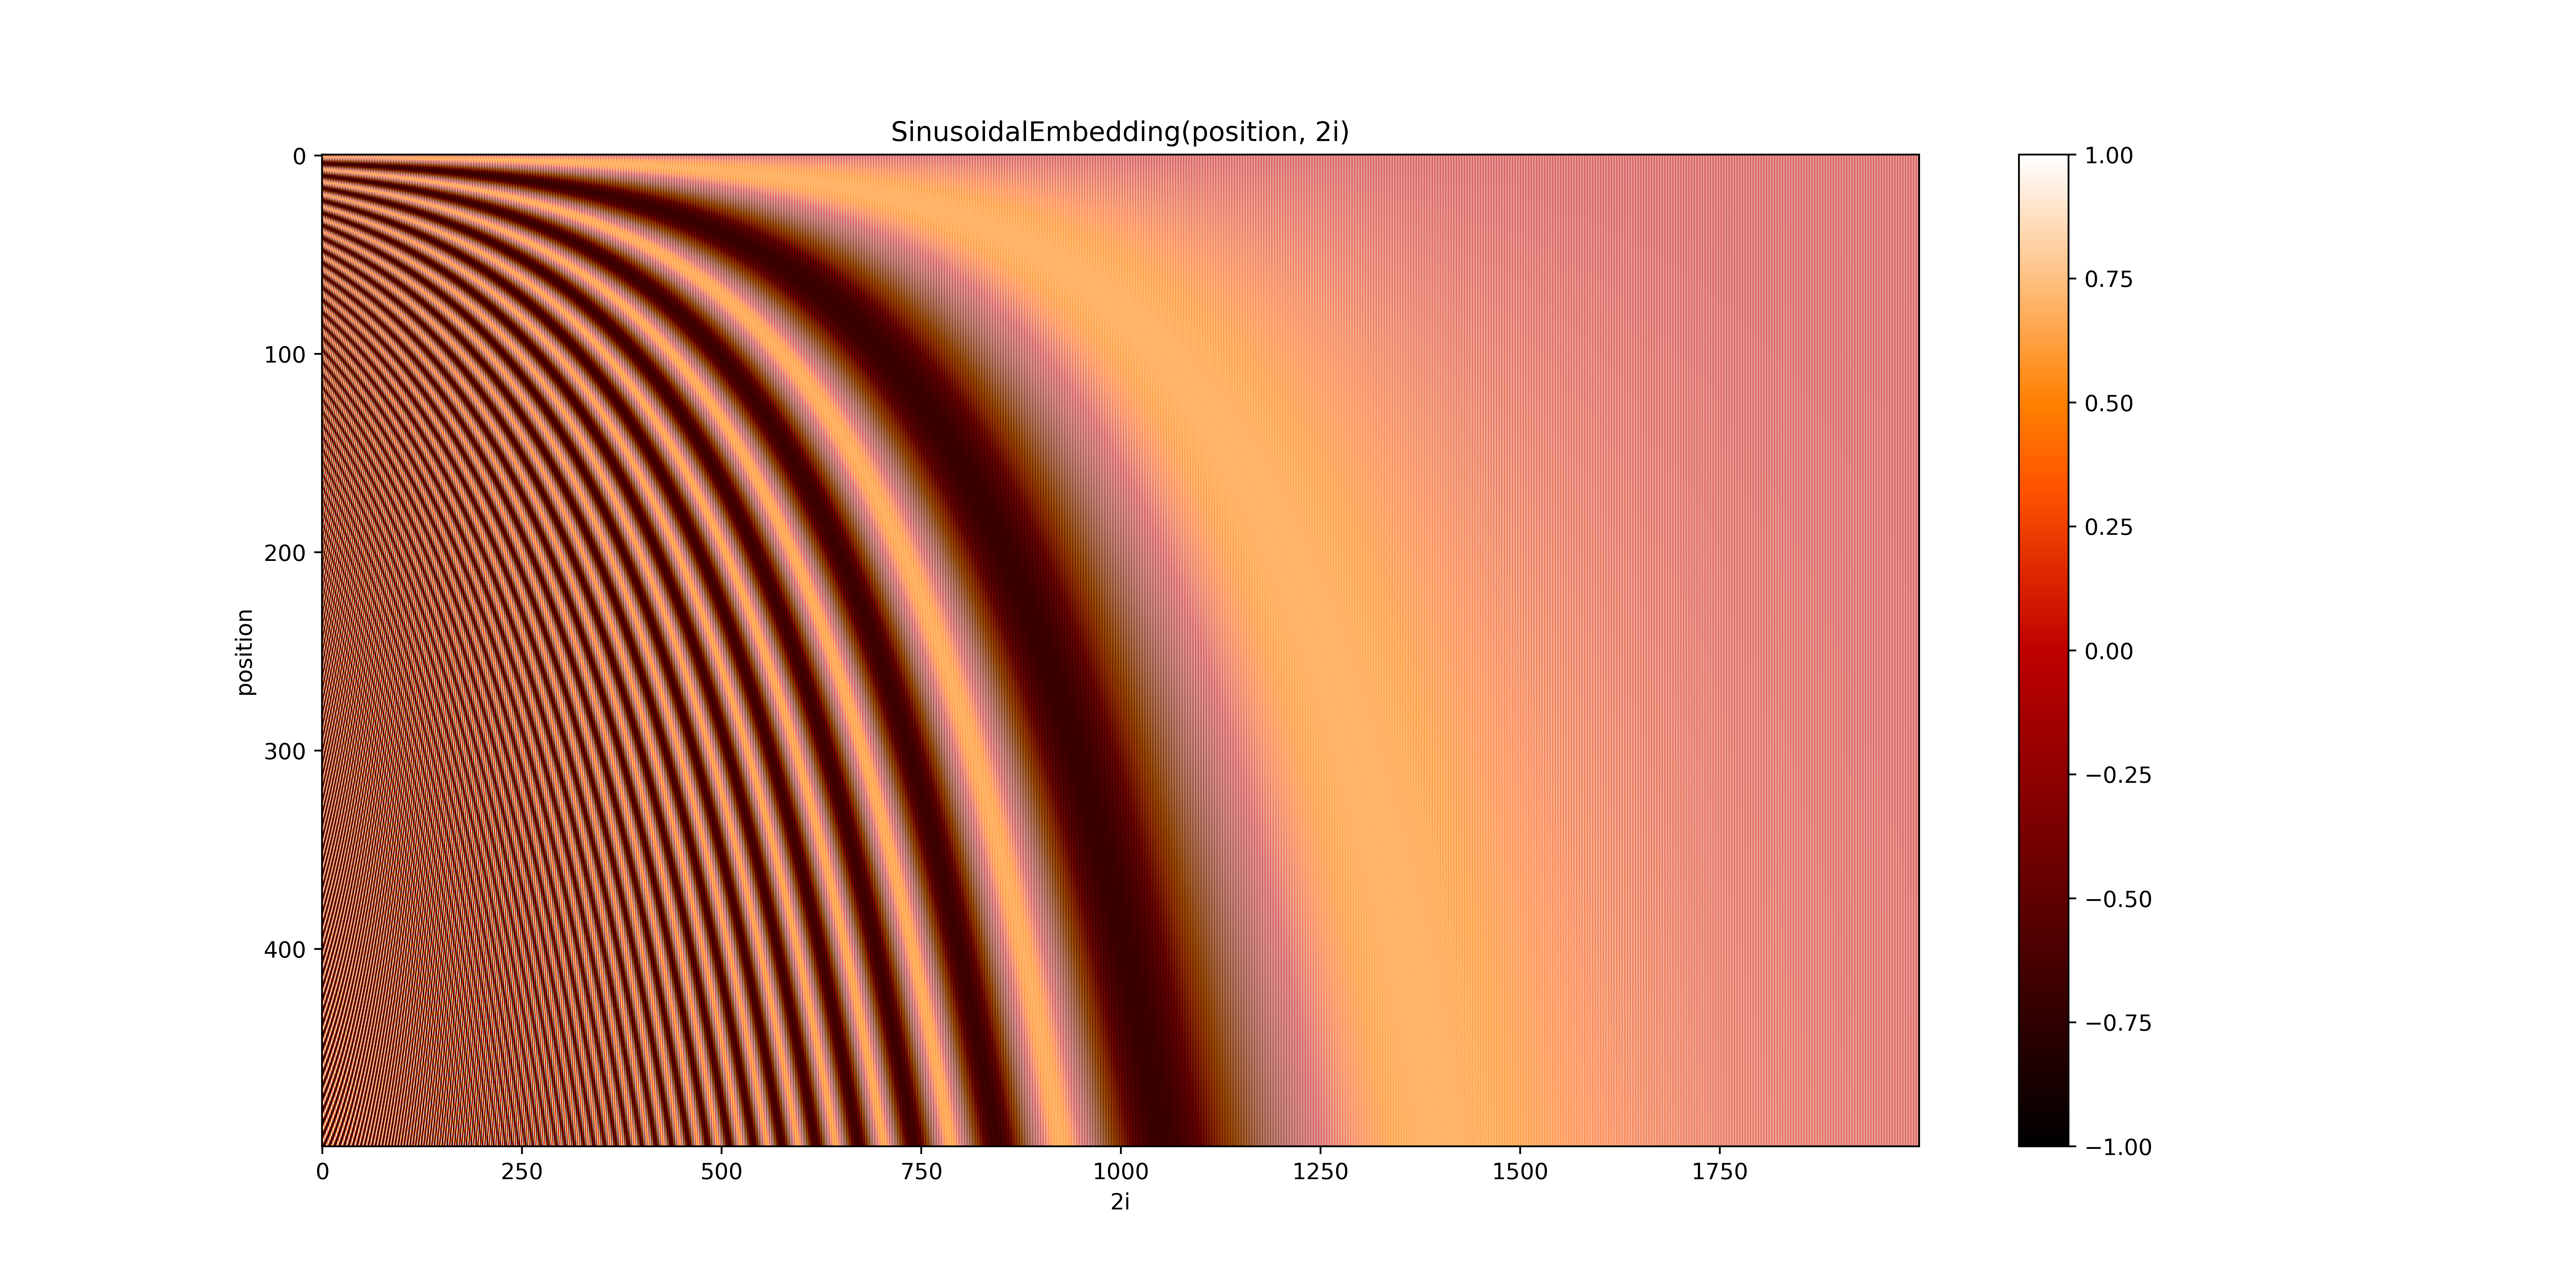
\includegraphics[width=\linewidth]{images/sin_embeds_freq_decay.png}
	\caption{The $SE$ function's frequency gets lower as the dimension grows}
	\label{fig:sin_embeds_freq_decay}
\end{figure}

In the plot above, we see that embeddings with close positions (two close values in the $pos$ axis) have different values of $SE(pos, 2i)$ for very small $2i$ (lower dimensions) while their values for higher dimensions are similar. On the other hand, if we pick two embeddings with very distant $pos$, they might differ from each other only in higher dimension. What this means is that in order to represent longer sentences (that contain positions very distant from each other), our model needs to have more dimensions. \textbf{The longer the input sentences, the higher the model's dimensions need to be.}

\subsection{Unique Representativiness ($SE$ is an injective function)}

Figure \ref{fig:sin_embeds_freq_decay} shows us that no two rows are the same because of the exponential decay of the frequencies with the increase of the dimension (increase of $2i$). As each row represents embeddings with different positions, what the figure is essentialy showing us is that two embeddings with different positions will never have the same representation, i.e., $SE$ is injective.

\subsection{Linearity \& Scale Invariance}

As previously mentioned, to be scale invariant, $SE$ must be such that the distance between $SE(pos)$ and $SE(pos + k)$ must be the same as the one between $SE(0)$ and $SE(k)$. In order to check that, we'll calculate the distance between every two sinusoidal embeddings of our module and see the linear property of such distance. Hence, all the rows will have to be subtracted from the first one, from the second one and so on up until the last one. 


\begin{lstlisting}[caption={Generating the plot of the module of the difference between every two different positions sinusoidal embeddings}]
	
import torch

# We'll create embeddings with many dimensions to better see the 
# frequency decay effect
max_pos = 1000
embed_dim = 1000


sinusoidal_embeddings = SinusoidalEmbeddings(max_pos, embed_dim).embeddings

# A single column tensor where each row's single element contains an 
# entire sinusoidal embeddings tensor
T_2 = sinusoidal_embeddings[:, None, :]

# A single row tensor where column's single element contains an 
# entire sinusoidal embeddings tensor
T_1 = sinusoidal_embeddings[None, :, :]

# By broadcasting, this operation will save the desired differences
# in the tensor's last dimension
differences = T_2 - T_1

# As the differences were saved in the last dimension, we need 
# to calculate the norm with respect to it, which is indicated 
# by dim=-1
distances = torch.norm(differences, p=2, dim=-1)

# Plot the resulting 2D tensor as a heatmap
plt.figure(figsize=(8, 6))
plt.imshow(distances.numpy(), aspect="auto", cmap="PuRd")
plt.colorbar(label="L2 Norm (Euclidean Distance)")
plt.xlabel("pos")
plt.ylabel("pos")
plt.title("Euclidean Distances Between Different Position Sinusoidal Embeddings")
plt.show()


\end{lstlisting}

\begin{figure}[h]
	\centering
	\includegraphics[width=\linewidth]{images/sin_embeds_scale_invariance.png}
	\caption{The sinusoidal embeddings difference vector's modules decrease linearly with the distance between the subtracted vectors}
	\label{fig:sin_embeds_scale_invariance}
\end{figure}

Figure \ref{fig:sin_embeds_scale_invariance} above shows us how the distance between sinusoidal embeddings of different positions decreases smoothly and linearly for embedidding with $d = 1000$.

%----------------------------------------------------------------------------------------

\end{document}
